\documentclass[12pt]{article}

\usepackage{amssymb, color}
\usepackage[cmex10]{amsmath}
\usepackage{xcolor,graphicx}
\usepackage[margin=1in]{geometry}
\usepackage{fancyhdr}
\usepackage{enumitem}

\usepackage[pdftex,bookmarks,letterpaper,hyperfigures,colorlinks
						,urlcolor=blue
						,citecolor=blue
						,linkcolor=blue
						,pagecolor=blue
						,pdfstartview=FitH]{hyperref}
\providecommand{\hreff}[1]{\href{http://#1}{http://#1}}
\providecommand{\email}[1]{\href{mailto:#1}{\textcolor{black}{#1}}}
\newcommand{\bbm}{\begin{bmatrix}}
\newcommand{\ebm}{\end{bmatrix}}

% Setup style for fancyheader
\pagestyle{fancyplain} % or fancyplain, plain

\lfoot{\textit{Last Modified: \today}}
\cfoot{}
\rfoot{\thepage}

\begin{document}
\begin{center}{\Large \bf{APMTH 50 Problem Set 2}} \vspace{0.2in}\\
{\large Due on Friday, March 3, by 5pm\\}
\end{center}

\subsection*{Collaboration policy}
Collaboration on homework and labs is
encouraged, but each student must write solutions in their own words, and not
copy them from anyone else.  Please write the name(s) of your collaborator(s) at the top of the homework.

\subsection*{Submission guidelines} Please upload your homework as a single Word or pdf document.   Unless stated otherwise, you do not need to include your code in your submission, but you should include all output (such as figures/plots) from your code. 

%\subsection*{Note} This homework has five problems.  The first four are below and the last one will be posted in an updated version of this document shortly.

\subsection*{Problems}
\begin{enumerate}
%\item question on DNA papers?
%\item question on inverse problems ...
\item Describe an inverse problem application that we have not talked about in class.  Write a few sentences about the problem, clearly stating the known and unknown quantities of the inverse problem.   You can come up with the problem on your own, or you can find a problem online or in other source.  Please cite all human and non-human sources.
\item Write a Matlab program that produces the $500 \times 500$ pixel color image below.  Your solution should include both your code and the output image from the code.
\begin{center}
  %\begin{longtable}{cc}
  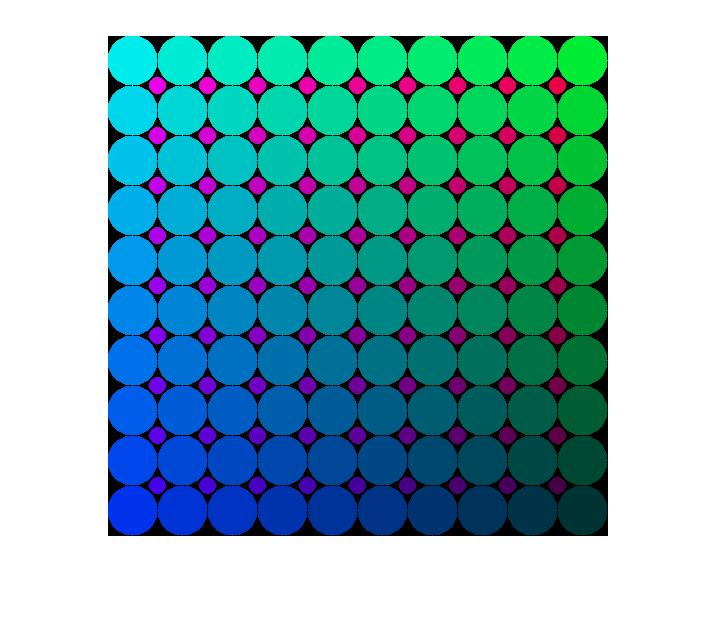
\includegraphics[width=.5\textwidth]{circletile} 
\end{center}
\newpage
\item %adapted from 2011, HW 4 v2, problem 2
The blue rectangle and white background have respective attenuation coefficients of 1 and 0 in units of inverse centimeters.  The dimension of each pixel is $\Delta x = \Delta y = 1$ cm.
\begin{center}
  %\begin{longtable}{cc}
  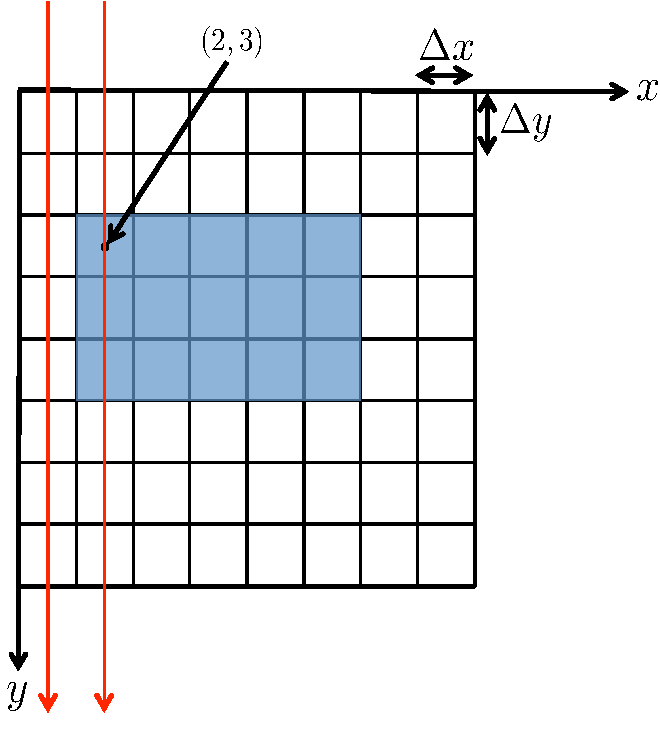
\includegraphics[width=.5\textwidth]{imagerectrays} 
\end{center}
\begin{enumerate}
\item  By hand, calculate the projections for rays that form $0, 45$, and $90$ degree angles with respect to the $y$-axis, and sketch the projections in each case.  Be sure to calculate eight values for each projection.  For example, for the $0$ degree projection, your rays should go through the center of each pixel in each column of the image matrix.  Two of the eight rays are marked by red lines in the figure.
\item  Without using Matlab's Radon transform function, write a program that creates the image, calculates the projections from part (a), and plots the projections. 
\end{enumerate}
\item The Radon transform of an object is given below.  Suppose the Radon transform of this object is the same for every angle $\theta$; that is, taking the Radon transform at any angle gives the projection below.   What could the object be?  Sketch the object.   Then generate the object in Matlab and calculate and plot the Radon transform for a few angles.  Please include your Matlab code in your submission.
%\begin{figure}[h]
\begin{center}
%  %\begin{longtable}{cc}
  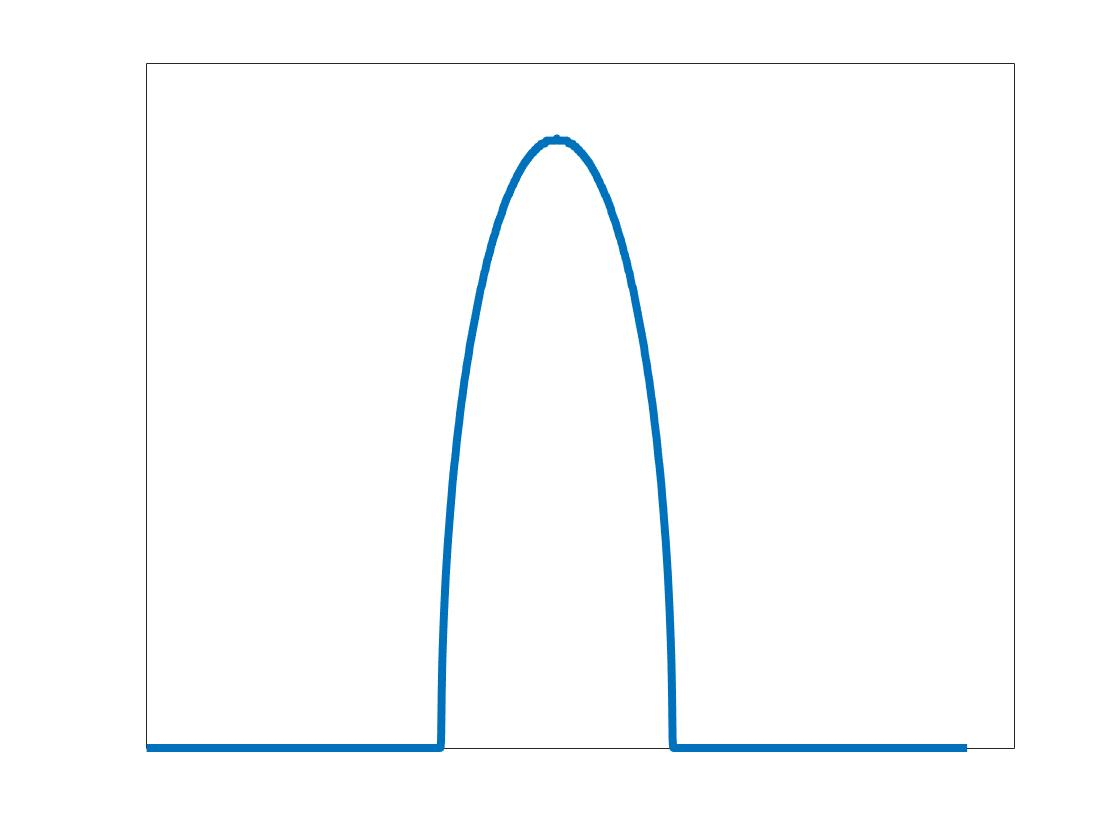
\includegraphics[width=.4\textwidth]{circle} 
 %  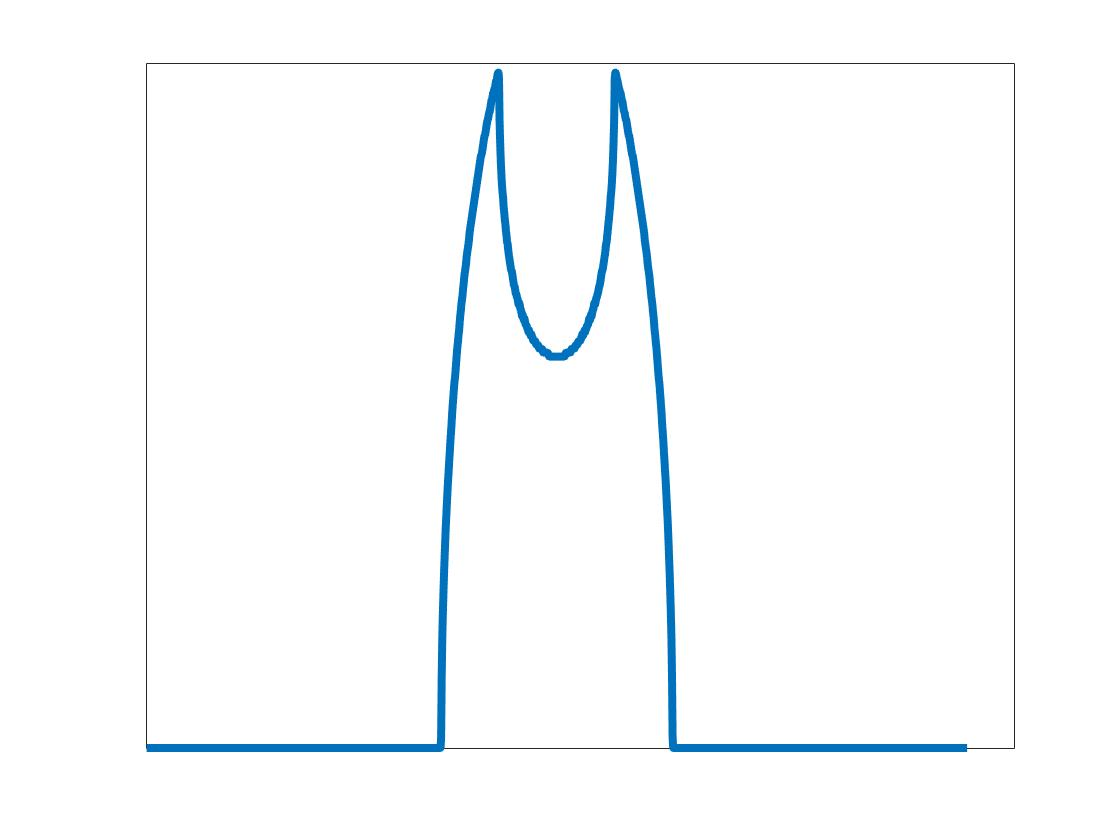
\includegraphics[width=.4\textwidth]{conc_circ} 
 % \caption{projection for object 1 and 2}
\end{center}
%\item This last problem will be posted shortly.  
\item In last week's lab, you used the command \verb+sinogram = radon(image, angles)+ to calculate the Radon transform of  \verb+image+ for a set of \verb+angles+.  Recall that each column of \verb+sinogram+ corresponded to the Radon transform of the object at a specified angle.  In this last problem we'll qualitatively explore \textit{backprojection}, one of the main methods for inverting the Radon transform and reconstructing an image for CT.    

\noindent Write a Matlab code to:
\begin{enumerate}
\item Create a $1000 \times 1000$ pixel black image with a white circle of radius 100 pixels at the center of the image.
\item Calculate the Radon transform with \verb+sinogram = radon(image, 0:dtheta:180)+ for \verb+dtheta = [90, 60, 45, 30, 15]+.  For each value of \verb+dtheta+, invert the transform to obtain a reconstructed version of the original image.  Please do this with a loop.
\item On one figure, create six subfigures: the original image from part (a) and the five reconstructed images from part (b).  Label each subfigure with the corresponding value of \verb+dtheta+.\\

\noindent Run the code and stare at the figure!  Notice that the reconstructed image gets better as more projections are used in the reconstruction.   Along with the circle at the center of the image, you should see stripes in the image at various angles.  These stripes are roughly the result of smearing each \textit{projection back} through the image along the rays in which it was originally acquired, so that all pixels along a particular ray are set to the same value.  If you click on the reconstructed image though, you'll notice that the pixels don't have the same values along the stripes.  This is because Matlab uses a more sophisticated type of backprojection to reconstruct the image, called \textit{filtered backprojection}, which is the most commonly used algorithm for CT systems. \\
\item Replace the image in part (a) by your house photo.  To do this, load your house photo, make it black-and-white, and convert it from \verb+uint8+ to \verb+double+.  Then re-run your code.  Are you satisfied with the reconstructed images?  Modify \verb+dtheta+ until you obtain a visually satisfactory reconstructed image.  

\end{enumerate}
%\begin{enumerate}
%\item The original image
%\item The reconstructed image
%\end{enumerate}

%\item question on matlab and radon transform and reconstruction
%\item %Estimate the number of hours it took  to complete the homework, excluding the time spent on the extra credit portions.
\end{enumerate}

\end{document}


